\chapter{Redes Ópticas Elásticas Multicore y Fragmentación del Ancho de Banda}
Las redes ópticas que se basan en WDM dividen el espectro de cada enlace en canales cuyo ancho de banda se fija de 50 GHz o 100 GHz. Esto debido a que la Unión Internacional de Telecomunicaciones (\textit{ITU-T International Telecommunication Union}) especificó el estándar G.694.1 en el año 2002.
%
Estas redes WDM resultan muy rígidas, y debido a eso es posible que ocurra una utilización ineficiente de la capacidad, provocado por el hecho de que el espacio entre dos canales adyacentes es relativamente grande y si la señal que se transmite utiliza un ancho de banda muy bajo, gran parte del espectro será desperdiciado.
%

Una nueva tecnología denominada Redes Ópticas Elásticas o \textit{Elastic Optical Networks} (EON) y su evolución: Las Redes ópticas Elásticas Multinúcleo o \textit{Multicore Elastic Optical Networks} (MC-EON) el cual no solo dividen el espectro óptico en Ranuras de Frecuencia o \textit{Frequency Slots} (FS) de 12.5 GHz conforme a lo establecido por el estándar definido en ITU-T (G.694.1) en el año 2012, sino que las (MC-EON) introducen un nuevo dominio de multiplexación espacial, al permitir la transmisión simultánea de múltiples señales ópticas en diferentes núcleos dentro de una misma fibra.
%
Esta aproximación multidimensional proporciona una mayor escalabilidad, eficiencia en la asignación del espectro y reducción del consumo energético, posicionando a las MC-EON como una de las tecnologías mas prometedoras para la implementación de redes ópticas de ultra alta capacidad en escenarios de próxima generación.
%

% En la Figura \ref{fig:eonwdm}, se muestra una comparación en la asignación de demandas en ambas tecnologías, observándose un mejor aprovechamiento del espectro óptico para el caso de las redes EON, debido a un menor desperdicio de ancho en banda.

% % \begin{figure}
% %     \centering
% %     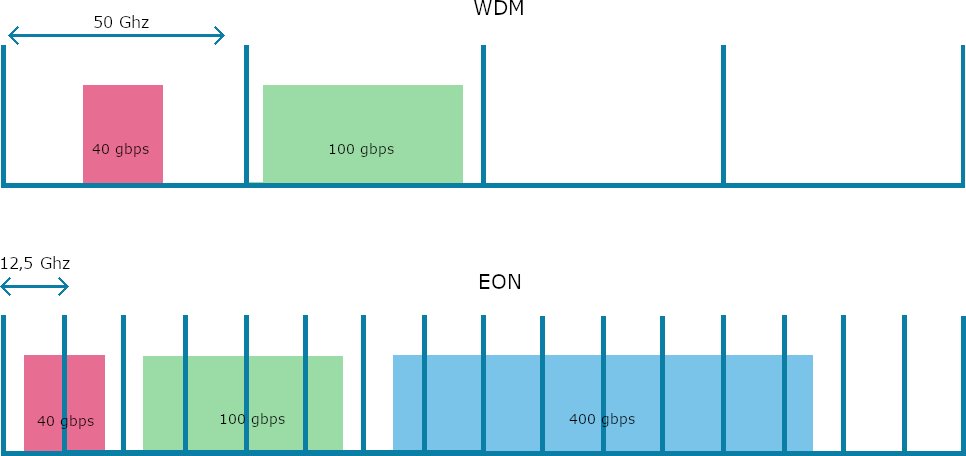
\includegraphics[width=0.95\textwidth]{capitulos/img/eonwdm.png}
% %     \caption{Redes WDM v s Redes EON}
% %     \label{fig:eonwdm}
% % \end{figure}


\section{Fragmentación del Ancho de Banda en MC-EON}
Las redes ópticas elásticas multinúcleo (MC-EON) permiten optimizar el uso del ancho de banda necesario para satisfacer una demanda, respetando tres restricciones fundamentales:
%

\begin{itemize}
    \item \textbf{Restricción de continuidad:} esta restricción implica que un cambio de luz o lightpath debe utilizar los mismos \textit{Frecuency Slots} (FS) a lo largo del camino establecido entre los nodos de origen y destino, tanto en la dimensión espectral como en la dimensión espacial (núcleo).
    \item \textbf{Restricción de consecutividad:} esta restricción establece que todos los FS utilizados para establecer un lightpath deben ser contiguos en el dominio espectral, formando un solo bloque contiguo de FS dentro del mismo núcleo. 
\end{itemize}
%

Estas restricciones conducen a que, tras sucesivas asignaciones y liberaciones de recursos, se genere la aparición de bloques aislados de FS no utilizados tanto en la dimensión espectral como en la dimesión espacial (núcleos) de los enlaces ópticos.
Dichos bloques fragmentados presentan desalineación tanto entre enlaces consecutivos de la ruta como entre los diferentes núcleos de una misma fibra multinúcleo. Como consecuencia, se incrementa significativamente la probabilidad de bloqueo de solicitudes, 
pudiendo la red rechazar demandas incluso cuando existe ancho de banda disponible suficiente en los enlaces. Este fenómeno se denomina \textbf{Fragmentación de la red} y en arquitecturas multinúcleo se manifiesta en dos domensiones complementarias:
%

\begin{itemize}
    \item \textbf{Fragmentación espectral:} se refiere a la presencia de bloques aislados de FS no utilizados en el dominio espectral, que no pueden ser aprovechados para establecer nuevas conexiones debido a las restricciones de continuidad y consecutividad.
    \item \textbf{Fragmentación espacial:} se refiere a la desalineación de bloques de FS disponibles entre los diferentes núcleos de una misma fibra multinúcleo, lo que dificulta la asignación eficiente de recursos en la dimensión espacial.
\end{itemize}
%

\textbf{Ejemplo ilustrativo del fenómeno:}
\begin{enumerate}[1 -]
   \item Se presenta el estado inicial del enlace mostrando las asignaciones activas de lightpaths distribuidos en los múltiples núcleos de la fibra.
   \item Se produce la liberación de recursos al finalizar el tiempo de vida de determinadas conexiones, generando segmentos espectrales disponibles dispersos en diferentes núcleos y posiciones del espectro.
   \item Se evidencia el rechazo de una nueva solicitud de conexión debido a que, pese a existir una cantidad agregada suficiente de FS libres en la red, estos no satisfacen simultáneamente las restricciones de contigüidad espectral dentro de un único núcleo y continuidad espacial a lo largo de la ruta. La conexión resulta bloqueada en todos los núcleos disponibles como resultado de la fragmentación tanto espectral como espacial inherente al sistema multinúcleo.  
\end{enumerate}
%

Para ilustrar estas restricciones, se presenta un ejemplo en las Figuras [] y [], donde se simula la conexión de una demanda de fod FS, con un nodo origen en 0 y un nodo destino en 3. En este escenario, existen dos posibblews caminos: 0-1-3 y 0-1-2-3.
%

La trayectoria de menor longitud corresponde a la ruta 0-1-3. No obstante, al procurar el establecimiento del lightpath mediante esta alternativa, la solicitud de conexión resulta denegada, dado que los enlaces 0-1 y 1-3 carecen de dos FS consecutivos y alineados espectralmente, tal como se evidencia en la Figura [].
%


\begin{figure}[H]
    \centering
    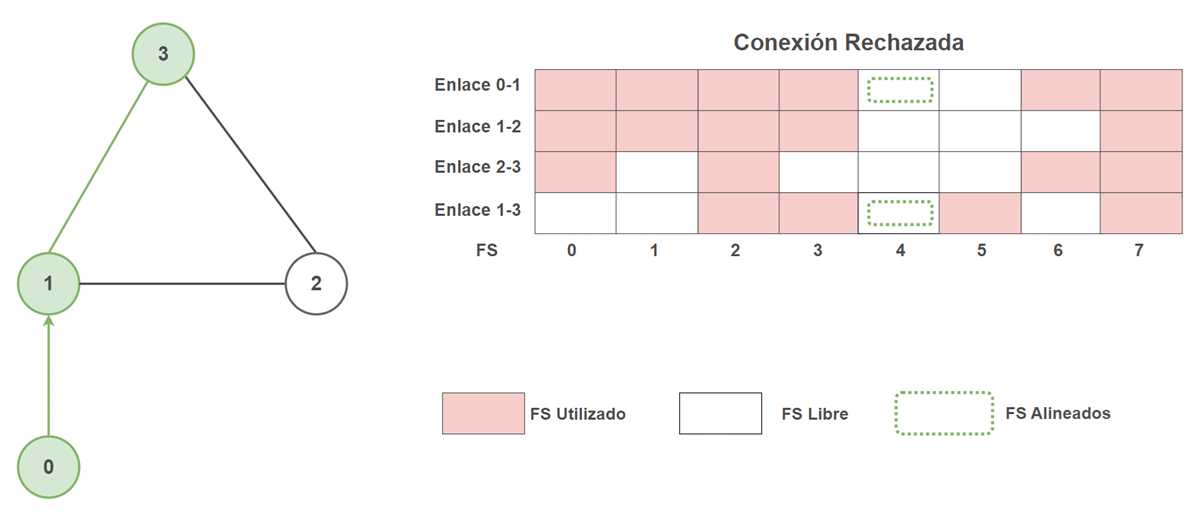
\includegraphics[width=1\textwidth]{capitulos/img/fragmentacionNuevo.png}
    \caption{Restricciones de contigüidad y continuidad aplicadas- Conexión Rechazada}
    \label{fig:fragmentacionNueva}
\end{figure}

\begin{figure}[H]
    \centering
    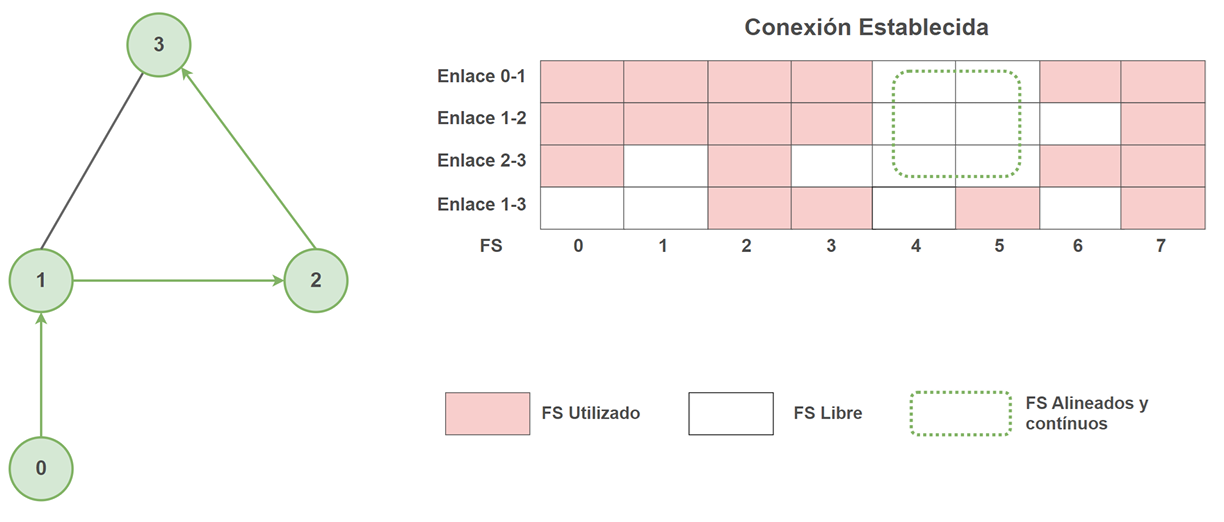
\includegraphics[width=1\textwidth]{capitulos/img/fragmentacion2Nuevo.png}
    \caption{Restricciones de contigüidad y continuidad aplicadas- Conexión Establecida}
    \label{fig:fragmentacion2Nueva}
\end{figure}

En contraste, al considerar la asignación del lightpath a través de la trayectoria de mayor extensión, específicamente 0-1-2-3, empleando los FS 4 y 5, la conexión se establece satisfactoriamente, puesto que esta configuración dispone de dos FS contiguos y alineados espectralmente, según se observa en la Figura [].
%

\subsection{Enfoques de gestión de fragmentación}
La problemática descrita previamente genera consecuencias perjudiciales para la infraestructura de red, ocasionando un incremento en la probabilidad de bloqueo y comprometiendo significativamente su desempeño óptimo y continuidad operacional. En consecuencia, resulta fundamental identificar estrategias que permitan prevenir, mitigar o reducir la fragmentación del espectro disponible.
%

De acuerdo con la bibliografía especializada, existen diversas aproximaciones que pueden ser consideradas para abordar la gestión de la desfragmentación. En la figura [] se presentan las principales estrategias de gestión de la fragmentación \cite{chatterjee2017fragmentation}.
%


La Desfragmentación constituye un procedimiento mediante el cual se ejecuta la reconfiguración o el re-ruteo de un subconjunto de conexiones existentes en la infraestructura de red. Su propósito fundamental consiste en reacomodar las asignaciones espectrales de las solicitudes de tráfico vigentes, consolidando de este modo los recursos disponibles en segmentos contiguos y continuos de mayor magnitud, los cuales pueden ser aprovechados para el establecimiento de futuras demandas \cite{talebi2014spectrum}.
%

Es factible abordar la problemática de la fragmentación prescindiendo de técnicas de desfragmentación espectral (Sin Desfragmentación), lo cual se alcanza mediante una administración del espectro orientada a la prevención de su fragmentación.
%

En el tratamiento de la fragmentación bajo un esquema Sin Desfragmentación, se pueden mencionar los algoritmos denominados Sensibles a la Fragmentación o \textit{Fragmentation Aware RSA} (FA-RSA). Estos consideran la fragmentación espectral durante el establecimiento de las demandas, empleando diversos indicadores de fragmentación, procurando así minimizar la fragmentación del espectro.
%

Alternativamente, es posible emplear técnicas de desfragmentación, las cuales se fundamentan en dos aproximaciones principales:
\begin{itemize}
         \item Desfragmentación Reactiva: El procedimiento se ejecuta como respuesta al bloqueo de una solicitud, con la finalidad de lograr su establecimiento exitoso.
         \item Desfragmentación Proactiva: Se lleva a cabo de manera periódica o en función de determinados umbrales que activan el proceso, permitiendo así reducir la fragmentación de la infraestructura de red y minimizar la ocurrencia de futuros bloqueos de solicitudes.
\end{itemize}
Las aproximaciones que implementan técnicas de desfragmentación pueden clasificarse además en: (i) estrategias sin re-ruteo, las cuales realizan únicamente una reasignación espectral en los \textit{lightpaths} o caminos ópticos establecidos, y (ii) estrategias con re-ruteo, que constituyen técnicas capaces de modificar tanto las rutas como el espectro asignado a los lightpaths existentes.
%

En el presente trabajo, para la gestión de la fragmentación se adoptó la aproximación con desfragmentación, de naturaleza proactiva y con re-ruteo de lightpaths preexistentes. En la figura [] se puede observar resaltada dicha estrategia.
%

\begin{figure}[H]
    \centering
    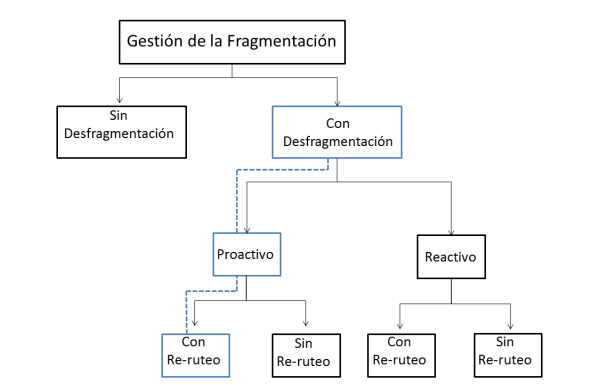
\includegraphics[width=1\textwidth]{capitulos/img/Gestion_Fragmentacion.PNG}
    \caption{Esquema de Gestión de la Fragmentación}
    \label{fig:gestion_fragmentacion}
\end{figure}
%


\section{Descripción del problema tratado}
La Fragmentación del Espectro en Redes Ópticas Elásticas Multinúcleo (Multi-Core EON) constituye una problemática que compromete la eficiencia en la utilización de recursos espectrales y espaciales. El desempeño de la infraestructura de red resulta severamente afectado, dado que este fenómeno puede ocasionar bloqueos de solicitudes debido a la ausencia de ranuras espectrales contiguas y alineadas entre enlaces consecutivos, así como por la indisponibilidad de núcleos adecuados, sin que necesariamente el espectro en todos los núcleos se encuentre completamente ocupado. En secciones previas se expusieron estrategias para el manejo de la fragmentación en la red; en el presente trabajo se examina la estrategia con desfragmentación, adoptando un enfoque proactivo.
%

Un método ampliamente implementado consiste en ejecutar el procedimiento de desfragmentación de manera periódica con el propósito de prevenir bloqueos futuros, abordando así una de las cuatro interrogantes planteadas por Zhang [], ¿Cuándo reconfigurar?.
%

En la figura [] se puede observar una posible solución a la problemática de la selección del momento óptimo para realizar la desfragmentación, la cual consiste en ejecutar desfragmentaciones periódicas en intervalos temporales fijos. En este caso, cada 100 unidades de tiempo, el eje vertical representa el volumen de tráfico cuantificado mediante el número de conexiones activas, mientras que el eje horizontal indica las unidades temporales; cada punto azul denota el instante en que el proceso de desfragmentación se ejecuta. Siguiendo este patrón, se evidencian situaciones donde se realizan procesos de desfragmentación cuando la red podría no requerirlos, considerando que la utilización de los recursos espectrales y de los núcleos constituye un indicador significativo del grado de fragmentación.
%

Además de la utilización de la red, existen otras métricas de fragmentación relevantes en redes multinúcleo, cuyos valores deben considerarse para el disparo de los procesos de desfragmentación, incluyendo la fragmentación por núcleo y la disponibilidad de recursos en la dimensión espacial.
%

De este modo, se evidencia la necesidad de un disparador inteligente para ejecutar el proceso de desfragmentación que considere todos estos parámetros o ``características'' para seleccionar apropiadamente el momento del disparo, dado que realizar múltiples desfragmentaciones de manera frecuente afecta directamente al desempeño de la red, pudiendo ocasionar disrupciones en las conexiones activas; mientras que ejecutar pocas desfragmentaciones muy dispersas resultaría en efectos prácticamente imperceptibles.
%

En síntesis, la selección del momento para ejecutar el proceso de desfragmentación resulta crítica debido a su impacto significativo en la cantidad de procesos de desfragmentación, lo cual incide directamente en las dos métricas globales más relevantes en el enrutamiento de redes ópticas elásticas multinúcleo: Cantidad de bloqueos y Cantidad de reconfiguraciones.
%

En los capítulos subsiguientes se presenta y aborda en profundidad un modelo de disparo inteligente que contempla numerosos factores tales como métricas de fragmentación de la red, utilización de recursos espectrales y espaciales, y bloqueos de solicitudes.
%

\begin{figure}[h!]
    \centering
    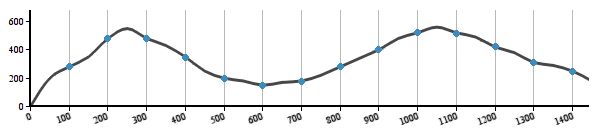
\includegraphics[width=1\textwidth]{capitulos/img/ejemploPeriodico.png}
    \caption{Ejemplo de desfragmentaciones periódicas con volumen de carga de tráfico variado}
    \label{fig:ejemploPeriodico}
\end{figure}
%


\section{Redes EON Multinúcleo}
Las redes EON Multinúcleo constituyen una variante avanzada de las redes EON que integran el concepto de fibras multinúcleo (MCF) para incrementar significativamente la capacidad de transmisión y la eficiencia espectral. Fundamentalmente, las redes EON Multinúcleo aprovechan múltiples núcleos independientes dentro de una misma fibra óptica para transmitir señales de forma simultánea y paralela, posibilitando una multiplicación de la capacidad de transmisión en comparación con las fibras convencionales [15].
 Estas características mencionadas en las EON Multinúcleo se materializan mediante la implementación de la Multiplexación por División de Espacio (SDM). Por esta razón, las redes EON Multinúcleo también se denominan SDM-EON[5]. En las redes EON Multinúcleo, se integra el concepto de asignación flexible de espectro con la utilización de múltiples núcleos, alcanzando una distribución más eficiente de la capacidad total de transmisión. Esta integración de tecnologías posibilita un incremento sustancial en la capacidad de transmisión a través de una única fibra, resultando esencial en un contexto donde la demanda de datos continúa creciendo de manera exponencial.
  Al incorporar el concepto de fibras multinúcleo en el diseño de las redes EON, se puede lograr una mayor adaptabilidad a las cambiantes necesidades del tráfico y una optimización más profunda de los recursos disponibles.
%

\begin{figure}[H]
    \centering
    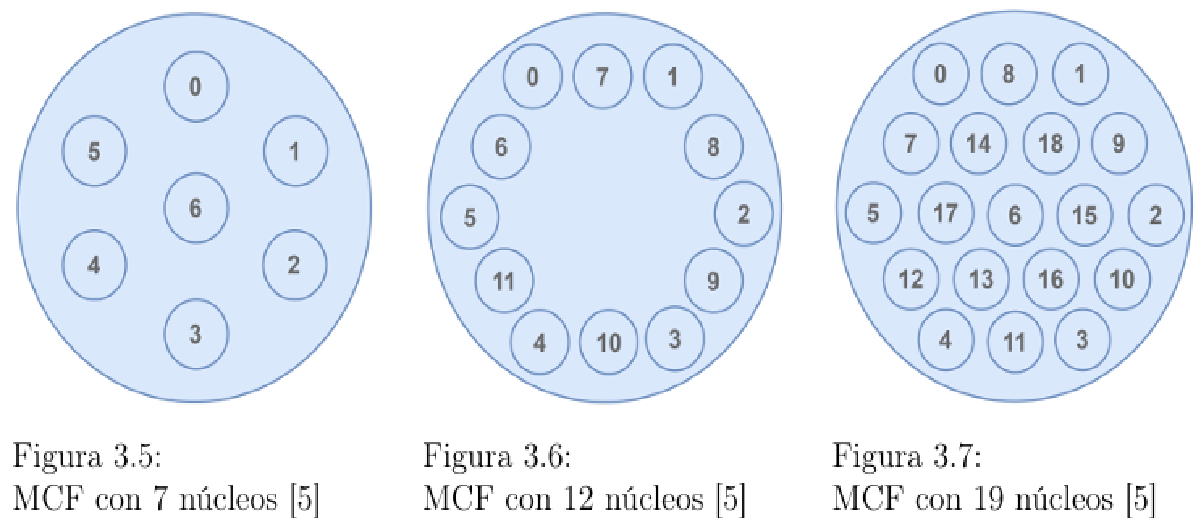
\includegraphics[width=1\textwidth]{capitulos/img/MCF_NUCLEOS.png}
    \caption{Ejemplo de Fibras Multinúcleo (MCF) con 7, 12 y 19 núcleos}
    \label{fig:MCF_NUCLEOS}
\end{figure}
%

Conforme a lo documentado en la literatura [], inicialmente podría considerarse que la utilización de redes EON con mayor cantidad de núcleos proporciona ventajas sustanciales debido a la amplia disponibilidad de recursos espectrales y espaciales. No obstante, se ha identificado que en las redes MCF, el principal desafío radica en la interferencia denominada diafonía (crosstalk), la cual se genera cuando una fracción de la potencia óptica de un núcleo se propaga hacia los núcleos contiguos.
 Este fenómeno ocasiona una interferencia significativa en los circuitos activos y complejiza considerablemente la asignación de las ranuras espectrales (FS). Investigaciones previas [] [] han indicado que para viabilizar la implementación de redes EON multinúcleo, resulta fundamental desarrollar fibras que minimicen la diafonía entre núcleos adyacentes.
%

 En la Figura [], se presenta una configuración de MCF con 7 núcleos dispuestos en un patrón hexagonal. En esta arquitectura, el núcleo central (núcleo N° 6) se encuentra rodeado por 6 núcleos adyacentes, resultando en una mayor incidencia de diafonía sobre este núcleo.
 En contraste, los núcleos periféricos (núcleos N° 0, 1, 2, 3, 4 y 5) poseen 3 núcleos adyacentes cada uno. La Figura [] exhibe una MCF con 12 núcleos organizados en una disposición anular. En esta configuración, cada núcleo presenta exactamente 2 núcleos adyacentes, lo que deriva en que todos los núcleos experimenten un nivel equivalente de diafonía.
 %

 Finalmente, la Figura [] ilustra una MCF con 19 núcleos. En este tipo de fibras, los núcleos pueden presentar hasta 6 núcleos adyacentes por núcleo, generando una mayor incidencia de diafonía.
%

\begin{figure}[H]
    \centering
    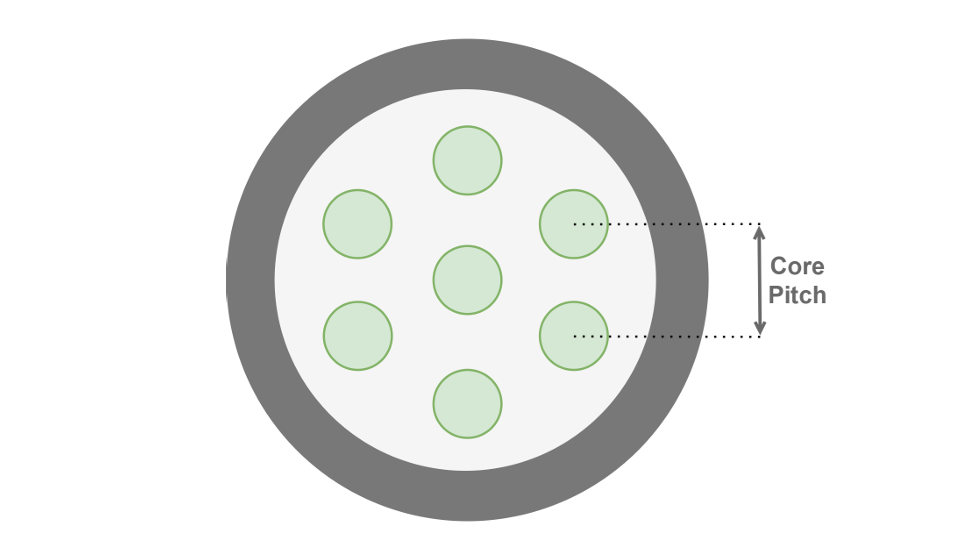
\includegraphics[width=1\textwidth]{capitulos/img/CORE_PITCH.png}
    \caption{Core Pitch entre dos núcleos adyacentes en un MCF de 7 núcleos}
    \label{fig:CORE_PITCH}
\end{figure}

\section{Diafonía en Redes Ópticas Elásticas Multinúcleo}
La diafonía constituye un fenómeno indeseado que se manifiesta en las redes de fibra óptica cuando la señal transmitida en una fibra se acopla hacia otra fibra contigua. En el contexto de las redes EON fundamentadas en MCF, la diafonía se define como la interferencia entre conexiones ópticas establecidas en núcleos adyacentes que emplean las mismas ranuras espectrales (FS) en un enlace común.
 Este tipo de interferencia se denomina diafonía entre núcleos o Inter-Core Crosstalk (XT). La interferencia ocasionada por el XT puede degradar la calidad de la señal en las FS afectadas, lo que implica que la señal en estas ranuras puede experimentar distorsiones, incrementando la probabilidad de errores en la transmisión de datos.
%
 
 Consecuentemente, impacta directamente en la capacidad de la red al «inhabilitar» estas FS para la transferencia de datos debido a la diafonía, generando espacios no utilizables entre ellas.
%

 En síntesis, esto deriva en una reducción de la cantidad total de FS disponibles para la transmisión de datos, limitando la capacidad operativa de la red. Con menor disponibilidad de FS, se reducen los canales para transmitir datos, lo que puede restringir la capacidad total de transmisión de la infraestructura de red.
%

 En las redes SDM-EON, el XT entre dos núcleos de una MCF depende significativamente de la distancia entre dicho par de núcleos, denominada core pitch ($\Lambda_{i,j}$). A mayor core pitch, menor será el impacto del XT entre estos dos núcleos [].
 No obstante, resulta importante destacar que, a medida que se incrementa el core pitch, la capacidad de la fibra óptica disminuye. Es decir, al aumentar la distancia física entre dos núcleos, se reduce el espacio disponible en la fibra óptica para albergar núcleos adicionales.
 Por consiguiente, resulta fundamental establecer un equilibrio entre un core pitch reducido para incrementar la capacidad y uno suficientemente amplio para minimizar los efectos del XT. Este balance posibilita optimizar el desempeño y la eficiencia de la red.
 %

\begin{figure}[H]
    \centering
    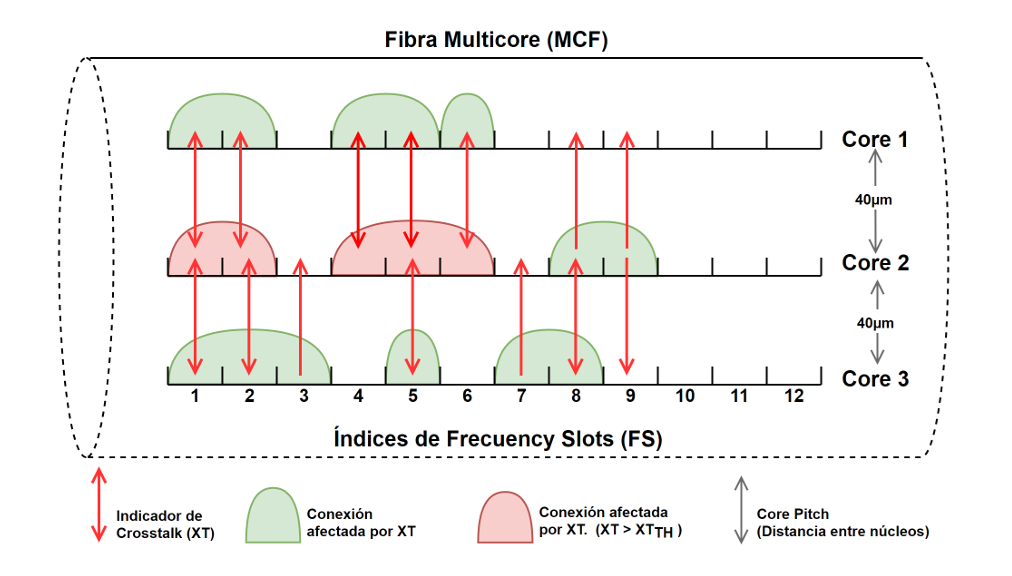
\includegraphics[width=1\textwidth]{capitulos/img/XT_MCF.png}
    \caption{XT en un Fibra MCF de 3 núcleos []}
    \label{fig:XT_MCF}
\end{figure}
%

Para demostrar el comportamiento del crosstalk (XT) entre núcleos en fibras multinúcleo, se analiza el ejemplo presentado en la figura [], la cual ilustra una fibra óptica multinúcleo (MCF) compuesta por tres núcleos organizados en configuración lineal.
En esta topología, resulta evidente que el núcleo central (núcleo 2) experimenta una interferencia significativa por XT intercore. Este fenómeno se atribuye a que ambos núcleos contiguos (núcleos 1 y 3) mantienen conexiones establecidas en intervalos espectrales similares a aquellos ya ocupados en el núcleo 2.
A modo de ejemplo, los segmentos espectrales FS1 y FS2 resultan inutilizables en el núcleo 2 debido a la interferencia generada por las asignaciones activas en los núcleos laterales.
Esta misma situación se replica en los intervalos FS4, FS5 y FS6 del núcleo mencionado. Consecuentemente, en arquitecturas SDM-EON basadas en fibras multinúcleo, resulta imperativo evaluar el impacto del XT intercore durante el proceso de asignación de recursos espectrales, a fin de mitigar degradaciones en la calidad de transmisión.

Es relevante destacar que el crosstalk intercore no afecta exclusivamente a los segmentos espectrales con demandas activas, sino también a aquellos recursos disponibles en núcleos adyacentes. Un análisis detallado de la figura [] revela que incluso los intervalos espectrales sin conexiones asignadas experimentan interferencia procedente de transmisiones en núcleos contiguos.
 Esto se ejemplifica con los segmentos FS8 y FS9 del núcleo 1, que sufren degradación por el XT generado desde las mismas posiciones espectrales en el núcleo 2. En determinadas circunstancias, esta interferencia puede superar el umbral de crosstalk admisible, imposibilitando la utilización de dichos recursos para el establecimiento de futuras conexiones en arquitecturas multinúcleo.

 %\section{Análisis Bibliográfico}     
% El trabajo presentado por M. Quagliotti \cite{quagliotti2017spectrum} propone un algoritmo RSA que busca mantener bajo el índice de fragmentación mediante el uso de una heurística básica durante la asignación del espectro, también brinda una amplia y útil descripción de métricas para evaluar la fragmentación del espectro.

% Para recopilar el conjunto de métricas de fragmentación utilizadas, realizaron un extenso estudio de la literatura científica, las cuales son: Utilization Entropy (UE), Shannon Entropy (SHF), External Fragmentation (EF), Access Blocking Probability (ABP), Compactness (SC) y High-slot Mark (HSM).

% Cada métrica de fragmentación proporciona su propia y peculiar medida de ocupación del espectro, relacionadas a la accesibilidad de recursos para el caso de EF, y ABP, grado de desorden y entropía en UE y SHF y compacidad del espectro ocupado en SC.

% Para nuestra investigación utilizamos algunas de las métricas presentadas en el mencionado articulo, las cuales nos sirven como características esenciales en la construcción de nuestro modelo de predicción de probabilidades de bloqueo.  

% Seguidamente presentamos un análisis bibliográfico de trabajos presentes en el estado del arte que abordaron el mismo problema.

% Jaume Comellas, Laura Vicario, y Gabriel Junyent \cite{comellas2018periodic} nos presentan un análisis de la desfragmentación periódica en redes EON con un tráfico dinámico, evaluando los diferentes efectos de los parámetros de desfragmentación en el rendimiento de la red.

% El enfoque presentado en el trabajo consiste en realizar las desfragmentaciones en periodos fijos de N unidades de tiempo, con el principal objetivo de encontrar valores adecuados de N, ya que periodos de desfragmetación muy pequeños implican tener el espectro tan compactado como sea posible, pero a expensas de ejecutar el algoritmo con demasiada frecuencia, lo cual añade complejidad al proceso. Por otro lado, para valores muy altos de N, los efectos de la desfragmentación son insignificantes.

% Este tipo de desfragmentaciones en periodos fijos es utilizado ampliamente en distintas investigaciones tales cómo \cite{davalos2019spectrum}, \cite{luo2012partial}, entre otros. En nuestra investigación utilizamos esta técnica a fin de comparar los resultados con el disparador que proponemos.

% Otra manera de afrontar el enfoque proactivo del proceso de desfragmentación es realizarlo mediante algún tipo de disparador de tal manera que la misma sea ejecutada solo en periodos de tiempo donde es realmente necesaria, a continuación, veremos algunos artículos los cuales usaron esta estrategia.

% La investigación realizada por Yutaka Takita y colegas \cite{takita2016wavelength} propone un mecanismo de disparo para el proceso de desfragmentación basado en el valor del \textit{High-slot Mark} (HM) el cual indica el número máximo de una ranura ocupada en la red. Utilizan esta métrica ya que lo consideran como una medida válida para evaluar la eficiencia en la utilización de los recursos. El proceso de desfragmentación se dispara de manera aleatoria cuando el valor del HM es mayor a un valor de \( HM_{max} \) definido previamente, en el artículo mencionado utilizan 30 como valor para \( HM_{max} \). 

% Para el proceso de disparo en nuestro método propuesto se utilizan un conjunto de características o parámetros que indican el estado actual de la red, parte de ellas al igual que el \textit{High-slot Mark} son también métricas que indican la fragmentación del espectro. En el capitulo 4 se explican en profundidad estas características donde una de ellas es el llamado \textit{Maximum Slot Index} (MSI) el cual tiene una definición equivalente al del \textit{High-slot Mark}. 

% Otra propuesta para el disparo es presentada por Ricardo V. Fávero y colegas \cite{favero2015new}. En su método combinan el enfoque reactivo y el enfoque proactivo para determinar el periodo en el que será ejecutado el proceso de desfragmentación, en la figura \ref{fig:favero} se puede observar el diagrama que ilustra el algoritmo propuesto.

% Inicialmente la variable \textit{d} que utilizan para representar el estado de fragmentación se coloca en 0, el proceso de desfragmentación (DS) se ejecuta al cumplirse alguna de las siguientes condiciones.

% Si se intenta establecer una demanda y no se encuentra un camino disponible para la misma, se verifica la variable \textit{d}, si esta se encuentra en 0 se ejecuta el proceso \textit{DS}, si no se logra establecer la demanda aun después del proceso de desfragmentación la misma se bloquea y la variable \textit{d} se cambia a 1.

% La otra posibilidad de ejecución es cuando se intenta liberar una demanda, se ejecuta el proceso \textit{DS} sí \textit{d} = 1 y si la cantidad de \textit{lighpaths} liberados (\textit{r}) es igual a la variable predefinida previamente \textit{R}. 

% Como se puede ver el método propuesto considera principalmente las conexiones liberadas por lo que puede considerarse como periódica.


% \begin{figure}[h!]
%     \centering
%     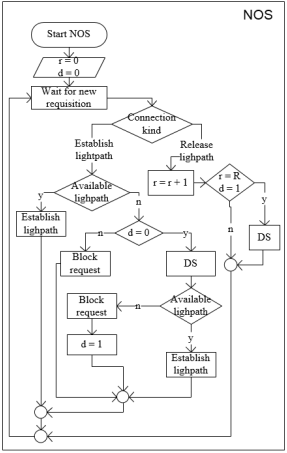
\includegraphics{capitulos/img/disparoFavero}
%     \caption{Algoritmo propuesto por Favero y colegas \cite{favero2015new}}
%     \label{fig:favero}
% \end{figure}

%Mingyang Zanhg y colegas plantean en su investigación \cite{zhang2013bandwidth} un disparo para el proceso de desfragmentación basado en la cantidad de conexiones liberadas. Básicamente consiste en ejecutar la desfragmentación cuándo la cantidad de conexiones liberadas es igual al parámetro fijo \textit{TH} (\textit{Threshold}). En su investigación utilizaron 300 como valor de \textit{TH}.

%El trabajo presentado por Jie Zhang y colegas \cite{zhang2012priority}, proponen un disparo basado en el concepto de \textit{Spectrum Compacteness} o Compacidad del Espectro (SC) el cual es una métrica de fragmentación.

%Para determinar el momento del disparo para el proceso de desfragmentación tienen en cuenta los siguientes pasos:  
% \begin{enumerate}[label=\arabic*)]
%     \item Seleccionar un valor apropiado de \textit{Spectrum Compactness} (SC) para actuar como umbral (T) para el disparo de la desfragmentación.
%     \item Actualizar el valor de SC después de liberar conexiones o al establecer una nueva conexión. 
%     \item Comparar los valores de SC y T; si SC < T disparar la desfragmentación y pasar al siguiente paso, sino volver al paso 2.
%     \item Actualizar el ultimo valor de SC después de la desfragmentación y volver al paso 3.
% \end{enumerate}

% Por último el trabajo propuesto por Zhang y colegas \cite{zhang2014dynamic} presentan un análisis del problema de la desfragmentación de redes EON dividido en cuatro sub-problemas, el tercero de ellos es ¿Cuándo reconfigurar?.

% Para el tercer subproblema plantean un algoritmo de disparo el cual tiene en cuenta la probabilidad de bloqueo instantánea (B) en un periodo \(\Delta \)t \((B(\Delta t))\) y la utilización del ancho de banda. 
% De esta forma buscan realizan la comparación entre \(B(\Delta t)\) con \(B_{th}\) (umbral de probabilidad de bloqueo para el disparo del proceso de desfragmentación) solo cuando la red se encuentra con un crecimiento en la utilización del ancho de banda. 
\newpage

